% !TeX root = ../main.tex

\chapter{Introduction}
\label{ch:introduction}

\paragraph*{Terminology Note}
Throughout this thesis, the artifact is referred to as a \textbf{game}. For pedagogical precision, it can also be categorized as a \textbf{serious game} and used as an instructional tool in educational contexts.
This terminology aligns with prior HPC educational activities explicitly framed as serious games~\citep{mullen2021teaching}.

%-----------------------------------------------------------------------
\section{Context and Motivation}
\label{sec:context-motivation}

%-----------------------------------------------------------------------
\subsection{The Challenge of Teaching High-Performance Computing}
\label{subsec:hpc-challenge}

High-Performance Computing (HPC) has become an indispensable tool in modern computational science, powering everything from weather forecasting and molecular dynamics simulations to machine learning and big data analytics. As computational problems grow in scale and complexity, the ability to write efficient parallel programs has transitioned from a specialized skill to a fundamental competency for software engineers and computational scientists.

However, teaching parallel computing concepts presents unique pedagogical challenges. Students frequently find it difficult to visualize how multiple threads or processes interact, communicate, and coordinate to solve problems efficiently. The principal challenges include:

\begin{itemize}
    \item \textbf{Abstraction Gap}: Concepts like threads, processes, synchronization, and message passing are inherently abstract and difficult to visualize
    \item \textbf{Cognitive Load}: Understanding parallel algorithms requires simultaneous consideration of multiple execution flows, shared resources, and synchronization primitives
    \item \textbf{Limited Immediate Feedback}: Traditional HPC assignments involve slow compile-submit-debug cycles that impede learning
    \item \textbf{Language Barriers}: HPC programming typically requires C/C++ or Fortran—languages with steep learning curves that can overshadow conceptual understanding. Students often struggle more with template errors and memory management than with parallelism itself due to the focus of C++ on keeping backwards compatibility as first priority
    \item \textbf{High Entry Barrier}: Setting up HPC environments and debugging distributed systems requires significant technical expertise that distracts from core concepts
\end{itemize}

Traditional lecture-based approaches struggle to convey the dynamic, interactive nature of parallel processes, motivating the exploration of alternative pedagogical approaches.

%-----------------------------------------------------------------------
\subsection{Serious Games as Educational Tools}
\label{subsec:serious-games}

\textbf{Serious games}---games designed with a primary purpose beyond entertainment---have emerged as powerful educational tools. By leveraging mechanics such as immediate feedback, progressive challenges, and interactive exploration, serious-game-based tools can make complex concepts more accessible and engaging.

\begin{itemize}
    \item \textbf{Active Learning}: Learners engage directly with concepts through interaction
    \item \textbf{Immediate Feedback}: Actions produce visible outcomes quickly
    \item \textbf{Visualization}: Abstract parallel behaviors become tangible
    \item \textbf{Safe Experimentation}: Risk-free environment for trial and error  without costly HPC infrastructure
    \item \textbf{Lower Entry Barrier}: Learners can focus on concepts before full programming complexity
\end{itemize}

%-----------------------------------------------------------------------
\subsection{From Physical Experiments to Digital Tooling}
\label{subsec:physical-experiments}

The pedagogical approach underlying this thesis stems from classroom experiments conducted by Professor Daniele D'Agostino, where students physically sorted numbered cards to simulate parallel computing paradigms:

\begin{itemize}
    \item \textbf{Sequential Execution}: A single student sorts all cards alone—demonstrating traditional sequential algorithms
    \item \textbf{OpenMP Simulation}: Multiple students work collaboratively at a shared desk with all cards visible in a common container, using public buffer areas for local sorting—demonstrating shared memory parallelism with partitioned per-thread work areas
\end{itemize}

These physical activities were highly effective at conveying parallel computing concepts in a tangible, memorable way. However, they faced significant limitations, including scalability (limited by desk size).

This thesis aims to capture that pedagogical effectiveness in a scalable, digital format accessible via web browsers, enabling students worldwide to experience similar learning benefits without the constraints of physical classrooms.

\begin{figure}[htbp]
    \centering
    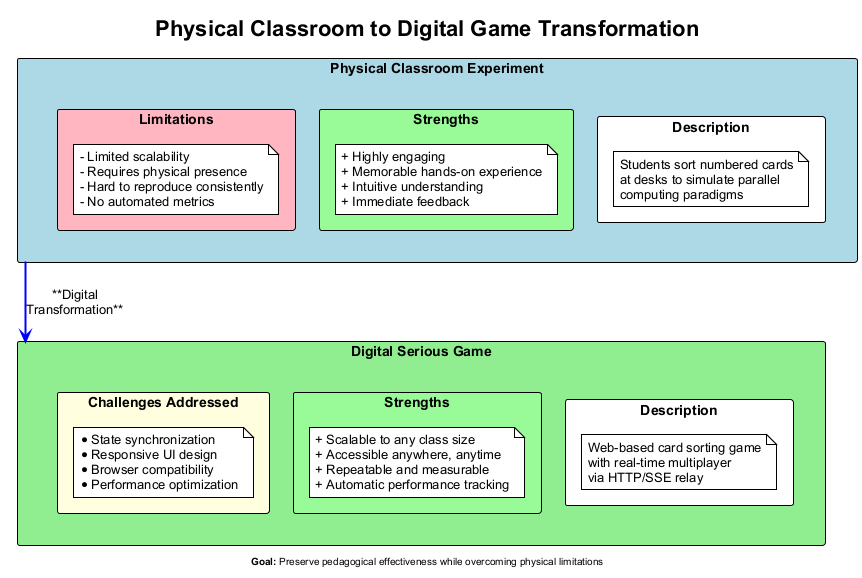
\includegraphics[width=0.85\textwidth]{figures/diagrams/physical-to-digital-mapping.png}
    \caption{Transformation from physical classroom activity to digital serious-game-based educational tool, preserving pedagogical effectiveness while overcoming physical limitations}
    \label{fig:physical-to-digital}
\end{figure}

%-----------------------------------------------------------------------
\section{Problem Statement}
\label{sec:problem-statement}

This thesis addresses the following research problem:

\begin{quote}
    \textit{How can we design and implement an effective web-based serious-game educational tool that teaches fundamental High-Performance Computing concepts (specifically OpenMP shared-memory parallelism and sequential vs. parallel execution) through interactive card-sorting while overcoming technical challenges of multiplayer state synchronization and responsive UI/UX constraints?}
\end{quote}

This overarching problem decomposes into three interrelated challenges:

\begin{itemize}
    \item \textbf{Educational Challenge}: How can abstract parallel computing concepts be mapped to concrete mechanics that accurately represent OpenMP paradigms?
    \item \textbf{Technical Challenge}: How can real-time multiplayer interaction be implemented across diverse devices with acceptable latency and consistent state?
    \item \textbf{Design Challenge}: How can we balance educational effectiveness with engagement and playability across different screen sizes and devices?
\end{itemize}

Detailed requirements analysis appears in Chapter~\ref{ch:methodology}.

%-----------------------------------------------------------------------
\section{Research Objectives}
\label{sec:objectives}

The primary objective of this thesis is to develop a functional serious-game-based educational tool that demonstrates the feasibility of teaching HPC concepts through web-based interactive activities, creating an open-source platform suitable for educational use and future research.

\subsection{Core Objectives}
\label{subsec:core-objectives}

\begin{enumerate}
    \item \textbf{Develop an Interactive Game-like Educational Tool}: Use card sorting as a metaphor for parallel sorting and OpenMP-style collaboration
    \item \textbf{Implement Web-First Functionality}: Run directly in modern browsers with responsive design
    \item \textbf{Create Multiplayer Capability}: Support many collaborative participants with synchronized shared state
    \item \textbf{Evaluate Technical Feasibility}: Assess architecture decisions and implementation challenges, including GDSync integration and HTTP/SSE relay networking
    \item \textbf{Support Instructor-Guided Use}: Ensure the artifact fits classroom and workshop workflows with facilitation and reflection
\end{enumerate}

%-----------------------------------------------------------------------
\section{Proposed Solution: HPC Sorting Serious Game}
\label{sec:proposed-solution}

This thesis presents the \textbf{HPC Sorting Serious Game}, a web-first serious-game-based educational tool for introducing parallel computing concepts through interactive card sorting. The card interaction model provides an intuitive bridge between concrete manipulation and abstract HPC concepts.
Technology selection process, alternatives explored, and final rationale are presented in Chapter~\ref{ch:methodology}.

%-----------------------------------------------------------------------
\section{Thesis Contributions}
\label{sec:contributions}

This thesis contributes to HPC education and educational game engineering in four areas:

\begin{enumerate}
    \item \textbf{Pedagogical Contribution}: A novel game-based approach for teaching OpenMP shared-memory parallelism and sequential vs. parallel execution comparison, directly inspired by successful physical classroom experiments, with systematic mapping between game mechanics and parallel computing paradigms. Additionally, demonstrates that fundamental HPC concepts can be taught effectively without requiring students to first master complex programming languages like C/C++, reducing cognitive load.
    \item \textbf{Technical Contribution}: A web-first implementation with synchronized multiplayer behavior and responsive UI for high-card-count interaction
    \item \textbf{Documentation Contribution}: Detailed discussion of practical engineering issues, including synchronization and framework constraints
    \item \textbf{Open-Source Contribution}: An extensible codebase that can be reused and expanded for future HPC education research
\end{enumerate}

Detailed discussion of these contributions appears in Chapter~\ref{ch:conclusion}.

%-----------------------------------------------------------------------
\section{Thesis Organization}
\label{sec:thesis-organization}

The remainder of this thesis is organized as follows:

\textbf{Chapter~\ref{ch:background}} reviews parallel computing fundamentals, serious games in education, web development constraints, and multiplayer architecture patterns.

\textbf{Chapter~\ref{ch:methodology}} describes the research method, requirements analysis, and technology selection.

\textbf{Chapter~\ref{ch:architecture}} presents system architecture, component design, networking model, and UI/UX strategy.

\textbf{Chapter~\ref{ch:implementation}} details implementation choices and key engineering decisions.

\textbf{Chapter~\ref{ch:problems}} analyzes development challenges and lessons learned.

\textbf{Chapter~\ref{ch:results}} presents system capabilities, technical performance, and preliminary educational observations.

\textbf{Chapter~\ref{ch:conclusion}} summarizes contributions and outlines future work.

\textbf{Appendices} provide supplementary materials including user documentation and technical references.

%-----------------------------------------------------------------------
